\documentclass{beamer}
\usepackage[latin1]{inputenc}

\usetheme{Madrid}
\usecolortheme{default}
\usepackage{amsmath}
\usepackage{amssymb,amsfonts,amsthm}
\usepackage{txfonts}
\usepackage{tkz-euclide}
\usepackage{listings}
\usepackage{adjustbox}
\usepackage{array}
\usepackage{tabularx}
\usepackage{gvv}
\usepackage{lmodern}
\usepackage{circuitikz}
\usepackage{tikz}
\usepackage{graphicx}
\usepackage{gensymb}
\usepackage{physics}

\setbeamertemplate{page number in head/foot}[totalframenumber]

\usepackage{tcolorbox}
\tcbuselibrary{minted,breakable,xparse,skins}



\definecolor{bg}{gray}{0.95}
\DeclareTCBListing{mintedbox}{O{}m!O{}}{%
  breakable=true,
  listing engine=minted,
  listing only,
  minted language=#2,
  minted style=default,
  minted options={%
    linenos,
    gobble=0,
    breaklines=true,
    breakafter=,,
    fontsize=\small,
    numbersep=8pt,
    #1},
  boxsep=0pt,
  left skip=0pt,
  right skip=0pt,
  left=25pt,
  right=0pt,
  top=3pt,
  bottom=3pt,
  arc=5pt,
  leftrule=0pt,
  rightrule=0pt,
  bottomrule=2pt,
  toprule=2pt,
  colback=bg,
  colframe=orange!70,
  enhanced,
  overlay={%
    \begin{tcbclipinterior}
    \fill[orange!20!white] (frame.south west) rectangle ([xshift=20pt]frame.north west);
    \end{tcbclipinterior}},
  #3,
}
\lstset{
    language=C,
    basicstyle=\ttfamily\small,
    keywordstyle=\color{blue},
    stringstyle=\color{orange},
    commentstyle=\color{green!60!black},
    numbers=left,
    numberstyle=\tiny\color{gray},
    breaklines=true,
    showstringspaces=false,
}
\title{4.11.3}
\date{14th september, 2025}
\author{Vishwambhar - EE25BTECH11025}

\begin{document}

\frame{\titlepage}
\begin{frame}{Question}
Find the equation of the line passing through (2,-1,2) and (5,3,4) and the equation of the plane passing through (2,0,3), (1,1,5), and (3,2,4). Also, find their point of intersection.
\end{frame}

\begin{frame}{Given}
Let:
\begin{align}
    \vec{P}_1=\myvec{2\\-1\\2};
    \vec{P}_2=\myvec{5\\3\\4}\\
    \vec{A}=\myvec{2\\0\\3};\vec{B}=\myvec{1\\1\\5};\vec{C}=\myvec{3\\2\\4}    
\end{align}
\end{frame}

\begin{frame}{Vector forms}
Direction vector of the line:
\begin{align}
    \vec{m}=\vec{P}_2-\vec{P}_1=\myvec{5\\3\\4}-\myvec{2\\-1\\2}=\myvec{3\\4\\2}
\end{align}

Vector form of the line can be written as:
\begin{align}
    \vec{x}=\vec{P}_1+\kappa\vec{m}
\end{align}

Vector form of the line can be written as:
\begin{align}
    \myvec{\vec{A}&\vec{B}&\vec{C}}^\top\vec{n}=\vec{1}\\
    \myvec{2&0&3\\1&1&5\\3&2&4}\vec{n}=\myvec{1\\1\\1}
\end{align}
\end{frame}

\begin{frame}{Augmented matrix}
Augmented matrix can be written as:
\begin{align}
    \augvec{3}{1}{2&0&3&1\\1&1&5&1\\3&2&4&1}R_2 \leftrightarrow R_1
    \augvec{3}{1}{1&1&5&1\\2&0&3&1\\3&2&4&1}\frac{R_2\rightarrow R_2-2R_1}{R_3\rightarrow R_3-3R_1}\\
    \augvec{3}{1}{1&1&5&1\\0&-2&-7&-1\\0&-1&-11&-2}\frac{R_2\leftrightarrow R_3}{R_2\rightarrow-R_2}\augvec{3}{1}{1&1&5&1\\0&1&11&2\\0&-2&-7&-1}
\end{align}
\end{frame}

\begin{frame}{Augmented matrix}
\begin{align}
    \frac{R_1\rightarrow R_1-R_2}{R_3\rightarrow R_3+2R_2}\augvec{3}{1}{1&0&-6&-1\\0&1&11&2\\0&0&15&3}R_3\rightarrow \frac{1}{15}R_3\\
    \augvec{3}{1}{1&0&-6&-1\\0&1&11&2\\0&0&1&\frac{1}{5}}\frac{R_1\rightarrow R_1+6R_3}{R_2\rightarrow R_2-11R_3}\augvec{3}{1}{1&0&0&\frac{1}{5}\\0&1&0&\frac{-1}{5}\\0&0&1&\frac{1}{5}}
\end{align}
\end{frame}

\begin{frame}{PLane}
Therefore, the plane equation is:
\begin{align}
    \myvec{1&-1&1}\vec{x}=5
    \vec{n}^\top\vec{x}=c
\end{align}

Substituting (4) in (11):
\begin{align}
    \vec{n}^\top\myvec{\vec{P}_1+\kappa\vec{m}}=c\\
    (\vec{n}^\top\vec{P}_1)+(\kappa\vec{n}^\top\vec{m})=c\\
    \kappa=\frac{c-(\vec{n}^\top\vec{P}_1)}{\vec{n}^\top\vec{m}}
\end{align}
\end{frame}


\begin{frame}{Point of intersection}
The point of intersection is (from(4)):
\begin{align}
    \vec{x}=\vec{P}_1+\brak{\frac{c-(\vec{n}^\top\vec{P}_1)}{\vec{n}^\top\vec{m}}}\vec{m}
\end{align}

Substituting the values from (11), (1) and (3):
\begin{align}
    \vec{x}=\myvec{2\\-1\\2}+\brak{\frac{0}{-3}}\myvec{3&4&2}\\
    \vec{x}=\myvec{2\\-1\\2}
\end{align}
\end{frame}


\begin{frame}[fragile]
    \frametitle{C Code}
    \begin{lstlisting}
#include <stdio.h>

int lpoint1[3] = {2, -1, 2};
int lpoint2[3] = {5, 3, 4};
int ppoint[3][4] = {{2, 0, 3, 1}, {1,1,5,1}, {3,2,4,1}};

int get_lpoint1(int index){
    return lpoint1[index];
}

int get_lpoint2(int index){
    return lpoint2[index];
}

int get_ppoint(int index1, int index2){
    return ppoint[index1][index2];
}
    \end{lstlisting}
\end{frame}

\begin{frame}[fragile]
    \frametitle{Python Code 1}
    \begin{lstlisting}
import ctypes
import numpy as np
import sympy as sp

lib = ctypes.CDLL("./problem.so")

lpoint=[0, 0, 0]
lvec=[0, 0, 0]

for i in range(0,3):
    lpoint[i] = lib.get_lpoint1(i)

for i in range(0,3):
    lvec[i] = lib.get_lpoint1(i) - lib.get_lpoint2(i)
    \end{lstlisting}
\end{frame}

\begin{frame}[fragile]
    \frametitle{Python Code 1}
    \begin{lstlisting}
print("Line equation is: ",lpoint,"+ k",lvec)

A = sp.Matrix([[2,0,3,1],
              [1,1,5,1],
              [3,2,4,1]])

rref, pivots = A.rref()

e = (rref[0,3],rref[1,3], rref[2,2])

print("Plane equation is: ", e[0],"x+",e[1],"y+",e[2],"/5z=",rref[0,0])
    \end{lstlisting}
\end{frame}

\begin{frame}[fragile]
    \frametitle{Python Code 2}
    \begin{lstlisting}
import numpy as np
import matplotlib.pyplot as plt
from mpl_toolkits.mplot3d import Axes3D


a, b, c, d = 1, -1, 1, 5   


xx, yy = np.meshgrid(np.linspace(-10, 10, 50), np.linspace(-10, 10, 50))


zz = (d - a*xx - b*yy) / c
    \end{lstlisting}
\end{frame}

\begin{frame}[fragile]
    \frametitle{Python Code 2}
    \begin{lstlisting}
p0 = np.array([2, -1, 2])   
v = np.array([3, 4, 2])    

t = np.linspace(-5, 5, 50)
x_line = p0[0] + v[0]*t
y_line = p0[1] + v[1]*t
z_line = p0[2] + v[2]*t


fig = plt.figure()
ax = fig.add_subplot(111, projection='3d')


ax.plot_surface(xx, yy, zz, alpha=0.5, color='cyan')    \end{lstlisting}
\end{frame}

\begin{frame}[fragile]
    \frametitle{Python Code 2}
    \begin{lstlisting}
ax.plot(x_line, y_line, z_line, color='red', linewidth=2)

ax.text(-12, -22, -8, r'$\frac{x-2}{3}=\frac{y+1}{4}=\frac{z-2}{2}$', fontsize=12, color="black")
ax.text(-14,21,12, "x-y+z=5", fontsize=12, color="black")
ax.text(2.1, -0.9, 2.1, "(2,-1,2)", fontsize=12, color="black")

ax.set_xlabel('X')
ax.set_ylabel('Y')
ax.set_zlabel('Z')

plt.savefig("../figs/plot.png")
plt.show()    \end{lstlisting}
\end{frame}

\begin{frame}{Plot}
    \begin{figure}
        \centering
        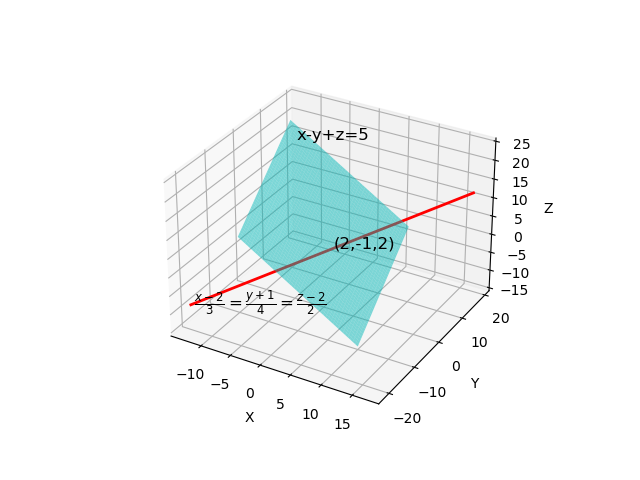
\includegraphics[width=0.5\columnwidth]{../figs/plot.png}
        \caption{Plot of given plane and line}
        \label{fig:fig}
    \end{figure}
\end{frame}
\end{document}
